\documentclass[a4paper]{article}

\usepackage[a4paper, top=8mm, bottom=8mm, left=8mm, right=8mm]{geometry}

\usepackage[english,russian]{babel}
\usepackage{fontspec}

%\usepackage{fontspec}
\setmainfont{FreeSerif}
\setsansfont{FreeSans}
\setmonofont{FreeMono}

\usepackage[tiny, compact]{titlesec}

\usepackage{titling}
\setlength{\droptitle}{-1cm}
\pretitle{\begin{center}\begin{bfseries}\Large}
\posttitle{\par\end{bfseries}\end{center}}
\preauthor{\begin{center}\normalsize}
\postauthor{\par\end{center}\vspace{-1.8cm}}

\usepackage{hyperref}
\usepackage{bookmark}
\usepackage{csquotes}
\usepackage{enumitem}
\usepackage{graphicx}
\usepackage{float}
\usepackage{booktabs}
% Для корректных ссылок на изображения с помощью \ref{...}
\usepackage{caption}
\captionsetup{hypcap=true}

\title{Оптимизация произведения Кронекера для библиотеки SuiteSparse:GraphBLAS}

\author{Арзамасцева Екатерина Андреевна}

\date{}

\begin{document}

\maketitle

\begin{flushright}
    Группа: \enquote{2025.Б72-мм}

    Кафедра: \emph{кафедра Системного программирования}

    Научный руководитель: \emph{кандидат физико-математических наук, доцент кафедры системного программирования Григорьев Семён Вячеславович}

    % А вот про консультанта укажите официальное место работы, с "ООО" или чем-то таким, и должностью желательно по трудовой, не просто "techlead". Выясните у консультанта.
    Консультант: \emph{Кутуев Владимир Александрович}
    
    Старший инженер-исследователь YADRO
    
    Номер семестра практики: \emph{2}
\end{flushright} 

\section{Постановка задачи}

Алгоритмы достижимости с ограничениями в виде контекстно-свободных языков, основанные на операциях линейной алгебры и использующиеся для статического анализа кода, могут быть основаны на произведении Кронекера~\cite{orachev2020}. При вычислении произведения Кронекера для разреженных матриц возникает проблема избыточного потребления памяти: результирующая матрица содержит большое число нулевых элементов, которые требуют выделения большого объема памяти. В актуальной версии библиотеки SuiteSparse:GraphBLAS~\cite{graphblas} фильтрация ненулевых элементов выполняется после построения результата, что приводит к высокому пиковому потреблению памяти и ограничивает применимость алгоритмов на больших графах.

\textbf{Целью работы является} добавление фильтрации нулевых элементов до этапа выделения памяти для результирующей матрицы в алгоритм произведения Кронекера с целью снижения пикового потребления памяти.

Результаты работы необходимы для повышения практической применимости алгоритмов, основанных на произведении Кронекера, для анализа больших графов.

\section{Описание предлагаемого решения}

В работе предложен алгоритм вычисления произведения Кронекера с ранней фильтрацией элементов. Основная идея заключается в предварительной оценке количества ненулевых значений результирующей матрицы и выделении памяти только под них. Таким образом, выделение памяти выполняется только под значащие элементы результата, что позволяет избежать избыточного потребления памяти~\cite{kutuev2023}.

Алгоритм адаптирован к актуальной версии библиотеки SuiteSparse:GraphBLAS и учитывает особенности её внутреннего представления разреженных матриц, в том числе используется JIT-компиляция, позволяющая уменьшить время вычисления произведения в сравнении с использованием обычных ядер.

\textbf{Реализация алгоритма:}

Для реализации ранней фильтрации используется двухпроходный алгоритм:
\begin{enumerate}
    \item \textbf{Первый проход:} подсчёт количества ненулевых элементов для каждого выходного вектора с использованием временных массивов.
    \item \textbf{Выделение памяти:} создание выходной матрицы C с точным размером \texttt{cnz} вместо верхней границы \texttt{cnzmax}.
    \item \textbf{Второй проход:} запись результата в выходную матрицу C с учётом пропуска нулевых элементов.
\end{enumerate}

\textbf{Изменение логики распараллеливания:}

В процессе реализации появилась проблема в логике распараллеливания для случая использования селектора с гиперразреженными матрицами. Исходная реализация использовала поэлементное распараллеливание, которое предполагало, что каждый элемент матрицы A генерирует ровно \texttt{bknz} записей в матрице C. Однако это предположение неверно для алгоритма с фильтрацией с гиперразреженной матрицей C. В оптимизированной версии осуществлён переход к векторному распараллеливанию, что устранило необходимость в сложных вычислениях смещений. Стоит отметить, что поэлементное распараллеливание позволяет более равномерно распределить нагрузку между потоками, вследствие чего может уменьшаться время вычисления произведения Кронекера. 

\textbf{Особенности работы с JIT-компиляцией:}

При попытке реализовать отдельное JIT-ядро для подсчета ненулевых элементов был добавлен JIT-шаблон, содержащий всю необходимую для этого логику. В результате экспериментов было установлено, что на generic ядрах (без использования JIT-ком\-пи\-ля\-ции) такой подход показывает себя хуже по времени выполнения (замедление на 120\%), чем версия, включающая эти расчеты в основной код функции (замедление на 40\%) по сравнению со стандартной реализацией. Затраты памяти при этом не меняются. Поэтому в итоговой реализации логика селектора встроена непосредственно в основной код, что обеспечивает лучшую производительность.

Реализация решения осуществлялась с использованием языка программирования C, библиотеки SuiteSparse:GraphBLAS.

\section{Эксперименты}

Проведённое экспериментальное исследование алгоритма показало, что на данных, характерных для различных задач статического анализа кода (например, alias analysis и points-to анализ), удаётся снизить пиковое потребление памяти, но это происходит за счёт увеличения времени выполнения операции по сравнению со стандартной реализацией, при сохранении корректности результатов и стабильности работы на различных наборах входных данных (графы программ и рекурсивные автоматы). Экспериментальное исследование заключалось в проведении 40 запусков алгоритма на входном наборе матриц, полученных в результате работы алгоритма статического анализа на реальных программах. Результаты замеров сгруппированы по названию анализируемого проекта (ось X графиков).  На графиках время неоптимизированной версии считается как сумма времени на вычисление Кронекера и время на фильтрацию ненулевых элементов. 

\textbf{Среда экспериментов:} 12th Gen Intel(R) Core(TM) i3-1215U.

Рассматривались две конфигурации оптимизированного алгоритма:
\begin{enumerate}
    \item Версия без JIT-компиляции (generic kernels)
    \item Версия с JIT-компиляцией
\end{enumerate}

\textbf{Результаты экспериментов:}

На рисунках~\ref{fig:v1}--\ref{fig:v2} представлены результаты экспериментов в виде box plot диаграмм, демонстрирующих распределение метрик для различных матриц. В таблицах~\ref{tab:summary_nojit}--\ref{tab:summary_jit} представлена сводная статистика по каждому типу графов.

\begin{figure}[H]
    \centering
    \includegraphics[width=0.9\textwidth]{images/rations\_generic.png}
    \caption{Результаты для версии без JIT}
    \label{fig:v1}
\end{figure}

\begin{table}[H]
    \centering
    \begin{tabular}{lccc}
        \toprule
        Граф & Среднее NNZ & Ускорение & Сокращение памяти \\
        \midrule
        avrora   & 30\,202\,599 & 0.698x & 2.29x \\
        eclipse  & 47\,956\,800 & 0.712x & 2.16x \\
        luindex  & 14\,375\,246 & 0.712x & 2.10x \\
        lusearch & 11\,141\,479 & 0.725x & 2.12x \\
        sunflow  &  9\,766\,410 & 0.699x & 2.37x \\
        \bottomrule
    \end{tabular}
    \caption{Сводная статистика для версии без JIT-компиляции}
    \label{tab:summary_nojit}
\end{table}

\begin{figure}[H]
    \centering
    \includegraphics[width=0.9\textwidth]{images/rations\_jit.png}
    \caption{Результаты для версии с JIT}
    \label{fig:v2}
\end{figure}

\begin{table}[H]
    \centering
    \begin{tabular}{lccc}
        \toprule
        Граф & Среднее NNZ & Ускорение & Сокращение памяти \\
        \midrule
        avrora   & 30\,202\,599 & 0.679x & 2.29x \\
        eclipse  & 47\,956\,800 & 0.703x & 2.15x \\
        luindex  & 14\,375\,246 & 0.707x & 2.09x \\
        lusearch & 11\,141\,479 & 0.715x & 2.11x \\
        sunflow  &  9\,766\,410 & 0.685x & 2.35x \\
        \bottomrule
    \end{tabular}
    \caption{Сводная статистика для версии с JIT-компиляцией}
    \label{tab:summary_jit}
\end{table}

\subsection{Анализ результатов:}

Эксперименты показали значительное снижение пикового потребления памяти для обеих версий оптимизированного алгоритма:
\begin{itemize}
    \item Версия без JIT: сокращение потребления памяти в 2.10--2.37 раза
    \item Версия с JIT: сокращение потребления памяти в 2.09--2.35 раза
\end{itemize}

Наибольшее снижение памяти наблюдается на графе sunflow.

При этом оптимизация приводит к увеличению времени выполнения, что является ожидаемым компромиссом:
\begin{itemize}
    \item Версия без JIT: ускорение 0.70--0.73x (замедление примерно на 37--43\%)
    \item Версия с JIT: ускорение 0.68--0.72x (замедление примерно на 39--47\%)
\end{itemize}

Увеличение времени обусловлено необходимостью двух проходов по данным вместо одного. JIT-версия обеспечивает сокращение времени выполнения по сравнению с generic версией (рис.~\ref{fig:v3}).

\begin{figure}[H]
    \centering
    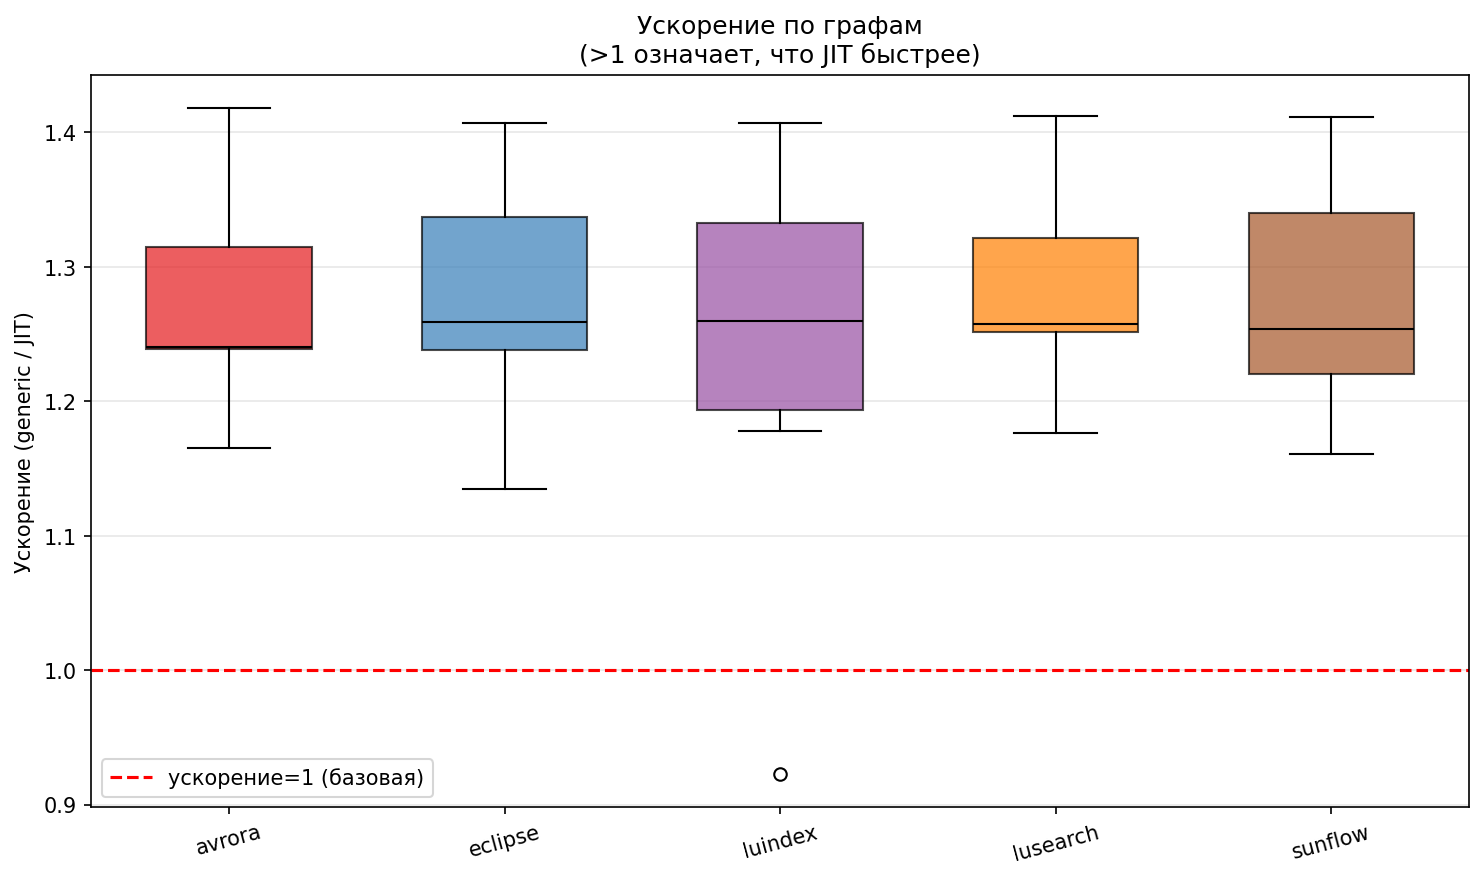
\includegraphics[width=0.9\textwidth]{images/time_comparison.png}
    \caption{Сравнение времени выполнения: JIT vs Generic}
    \label{fig:v3}
\end{figure}

\subsection{Выводы из экспериментов:} Предложенная оптимизация успешно решает поставленную задачу снижения пикового потребления памяти, что особенно важно для анализа больших графов программ. Увеличение времени выполнения является приемлемым компромиссом, так как во многих сценариях статического анализа ограничение по памяти является более критичным фактором, чем время выполнения.

\section{Заключение}

В ходе выполнения работы получены следующие результаты:

\begin{itemize}
    \item Добавлена фильтрация нулевых элементов на этапе вычисления в алгоритм произведения Кронекера для разреженных матриц в SuiteSparse:GraphBLAS.
    \item Реализован двухпроходный алгоритм с предварительным подсчётом ненулевых элементов и выделением памяти только под значащие элементы результата.
    \item Достигнуто снижение пикового потребления памяти произведением Кронекера в 2.1--2.4 раза на различных наборах данных из области статического анализа кода.
    \item Алгоритм адаптирован к актуальной версии библиотеки SuiteSparse:GraphBLAS.
    \item Проведённое экспериментальное исследование подтвердило эффективность оптимизации по памяти при приемлемом увеличении времени выполнения.
\end{itemize}

Решение не является финальным и открывает направления для дальнейшей работы:
\begin{itemize}
    \item Добавление возможности использования JIT-компиляции на этапе подсчета ненулевых элементов результирующей матрицы с целью сокращения времени подсчета.
    \item Добавление возможности отбирать ненулевые элементы по пользовательскому критерию вместо использующейся сейчас побайтовой проверки на 0.
\end{itemize}

Pull Request: \url{https://github.com/kijexs/GraphBLAS/pull/2}

\begin{thebibliography}{9}
\bibitem{orachev2020}
Orachev, E., Epelbaum, I., Azimov, R., Grigorev, S. (2020). Context-Free Path Querying by Kronecker Product. In: Darmont, J., Novikov, B., Wrembel, R. (eds) Advances in Databases and Information Systems. ADBIS 2020. Lecture Notes in Computer Science, vol 12245. Springer, Cham. https://doi.org/10.1007/978-3-030-54832-2\_6

\bibitem{graphblas}
Исходный код библиотеки SuiteSparse:GraphBLAS [Электронный ресурс]. URL: \url{https://github.com/SparseLinearAlgebra/GraphBLAS}.

\bibitem{kutuev2023}
Experimental investigation of context-free-language reachability algorithms as applied to static code analysis / Kutuev Vladimir. URL: \url{https://dspace.spbu.ru/items/36014e9c-fae5-4793-9f17-7c1ddfc3421c}.
\end{thebibliography}

\end{document}
